\begin{figure}[htb]
	\centering
	\begin{minipage}[c]{.45\linewidth}
		\centering
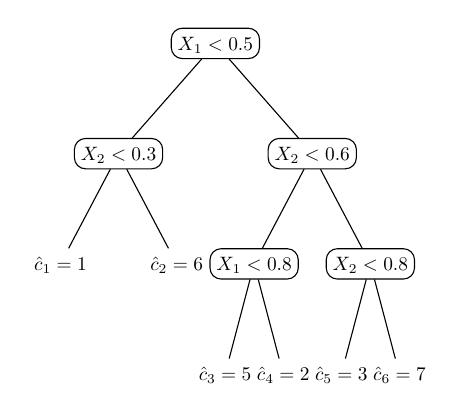
\begin{tikzpicture}[
scale = 0.7,
every node/.style={transform shape},
baseline,
level distance=20mm,
text depth=.1em,
text height=.8em,
level 1/.style={sibling distance=10em},
level 2/.style={sibling distance=6em},
level 3/.style={sibling distance=3em}]


\node [rounded corners, draw] {$X_1 < 0.5$}
child {node [rounded corners, draw] {$X_2 < 0.3$}
	child {node {$\hat{c}_1=1$}}
	child {node {$\hat{c}_2=6$}}
}
child {node [rounded corners, draw] {$X_2 < 0.6$}
	child {node [rounded corners, draw] {$X_1<0.8$}
		child {node {$\hat{c}_3=5$}}
		child {node {$\hat{c}_4=2$}}
	}
	child {node [rounded corners, draw] {$X_2<0.8$}
		child {node {$\hat{c}_5=3$}}
		child {node {$\hat{c}_6=7$}}
	}
};

\end{tikzpicture}
		\subcaption{Regression Tree based on initial data set.}
	\end{minipage}%
	\hfill%
	\begin{minipage}[c]{.45\linewidth}
		\centering
		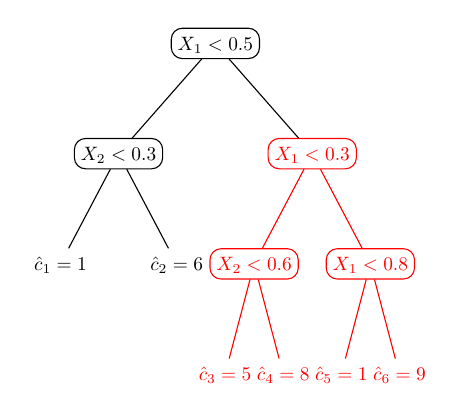
\begin{tikzpicture}[
scale = 0.7,
every node/.style={transform shape},
baseline,
level distance=20mm,
text depth=.1em,
text height=.8em,
level 1/.style={sibling distance=10em},
level 2/.style={sibling distance=6em},
level 3/.style={sibling distance=3em}]


\node [rounded corners, draw] {$X_1 < 0.5$}
child {node [rounded corners, draw] {$X_2 < 0.3$}
	child {node {$\hat{c}_1=1$}}
	child {node {$\hat{c}_2=6$}}
}
child {node [red, rounded corners, draw] {$X_1 < 0.3$}
	child [red] {node [rounded corners, draw] {$X_2<0.6$}
		child {node {$\hat{c}_3=5$}}
		child {node {$\hat{c}_4=8$}}
	}
	child [red] {node [rounded corners, draw] {$X_1<0.8$}
		child {node {$\hat{c}_5=1$}}
		child {node {$\hat{c}_6=9$}}
	}
};

\end{tikzpicture}
		\subcaption{Regression Tree based on perturbed data set.}
	\end{minipage}
	\caption[Illustration of the instability of Regression Trees.]{Illustration of the instability of Regression Trees.}
	\label{fig:Tree_Instability}
	
\end{figure}


